\section{Qualitative Analysis}
\label{sec:qualitative_analysis}

We present qualitative comparisons of our UniCL-AffSeg framework against the WeCLIP baseline and ground truth annotations on selected Pascal VOC 2012 images. Both class activation maps (CAMs) and pseudo-labels are visualized to highlight differences in object localization, boundary delineation, and overall mask quality.

\subsection{Selection of Examples}
The images were chosen to represent a variety of scenarios, including: 
\begin{itemize}
    \item \textbf{Easy cases:} Large, isolated objects where CAMs are expected to cover most of the object region.
    \item \textbf{Challenging cases:} Small objects, occlusions, or cluttered backgrounds where weakly supervised CAMs often fail to capture complete object extents.
\end{itemize}

\subsection{Visualization Layout}
Figure~\ref{fig:qualitative_comparison} shows the qualitative results in a structured grid. 
The first row presents the input image, ground truth, WeCLIP CAM, and our CAM, while the second row shows the corresponding pseudo-labels generated by WeCLIP and our method. This layout allows a direct comparison of both intermediate activations and the resulting segmentation masks.


\begin{figure}[ht]
  \centering
  \setlength{\tabcolsep}{2pt} % adjust spacing
  \renewcommand{\arraystretch}{0.9}

  % CAMs with class labels on the left
  \begin{tabular}{c c c c} % first column = label
    % Column headers
    & (a) Input & (b) WeCLIP & (c) Ours \\[1mm]

    % First example
    \textbf{Cat} &
    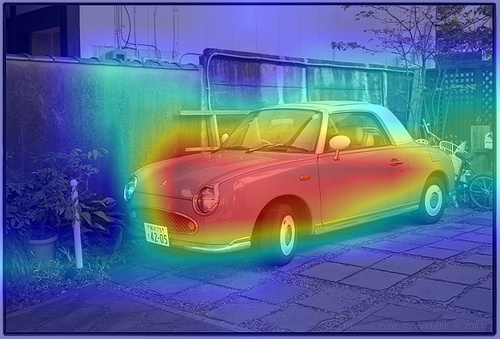
\includegraphics[width=0.23\textwidth]{figures/qualitative_analysis/test_cam/2010_005860_6.jpg} &
    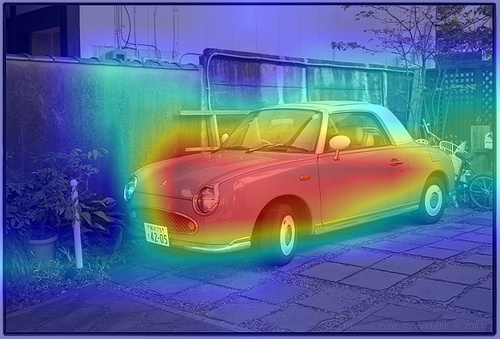
\includegraphics[width=0.23\textwidth]{figures/qualitative_analysis/test_cam/2010_005860_6.jpg} &
    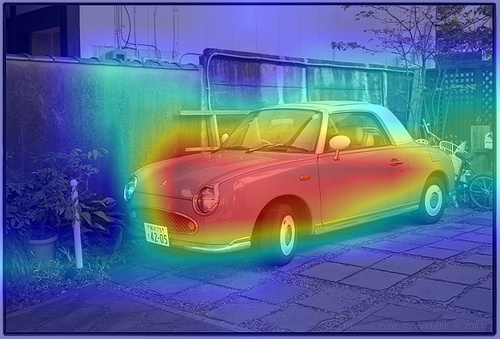
\includegraphics[width=0.23\textwidth]{figures/qualitative_analysis/test_cam/2010_005860_6.jpg} \\

    % Second example
    \textbf{Dog} &
    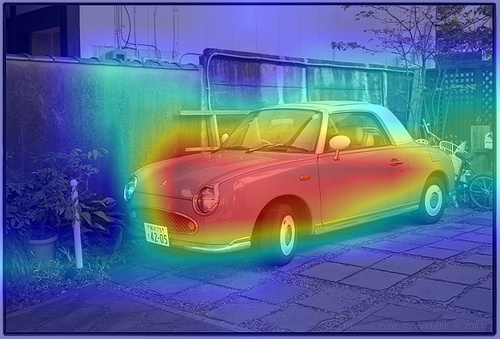
\includegraphics[width=0.23\textwidth]{figures/qualitative_analysis/test_cam/2010_005860_6.jpg} &
    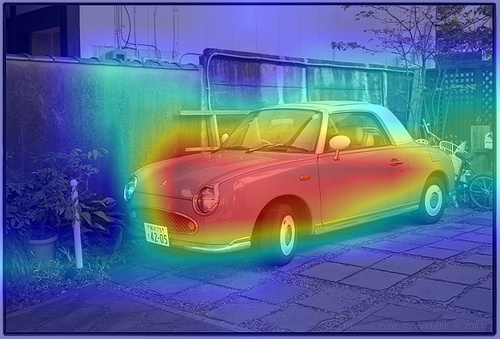
\includegraphics[width=0.23\textwidth]{figures/qualitative_analysis/test_cam/2010_005860_6.jpg} &
    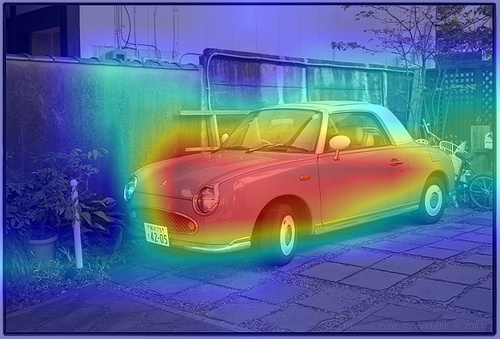
\includegraphics[width=0.23\textwidth]{figures/qualitative_analysis/test_cam/2010_005860_6.jpg} \\
  \end{tabular}

  \caption{Qualitative comparison of CAMs between WeCLIP and our UniCL-AffSeg on PASCAL VOC 2012 \textit{val} set. The class label for each image is shown on the left.}
  \label{fig:qualitative_comparison_cam_val}
\end{figure}

\begin{figure}[ht]
  % Pseudo-labels
  \begin{tabular}{cccc}
    (a) Input & (b) GT & (c) WeCLIP & (d) Ours \\

    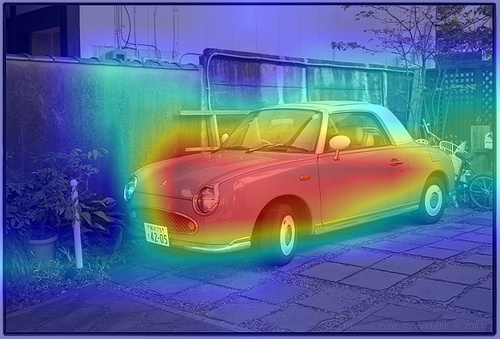
\includegraphics[width=0.22\textwidth]{figures/qualitative_analysis/test_cam/2010_005860_6.jpg} &
    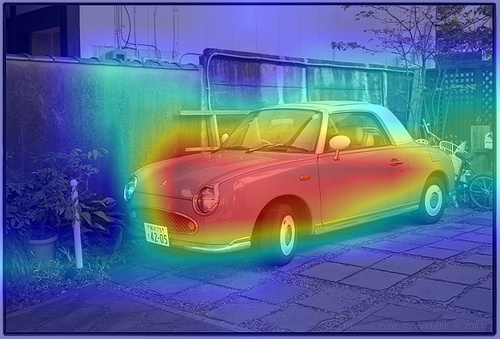
\includegraphics[width=0.22\textwidth]{figures/qualitative_analysis/test_cam/2010_005860_6.jpg} &
    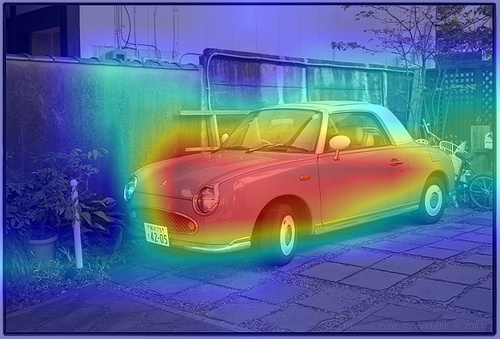
\includegraphics[width=0.22\textwidth]{figures/qualitative_analysis/test_cam/2010_005860_6.jpg} &
    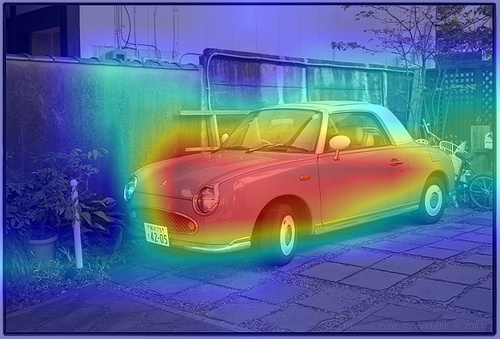
\includegraphics[width=0.22\textwidth]{figures/qualitative_analysis/test_cam/2010_005860_6.jpg} \\
  \end{tabular}

  \caption{Qualitative comparison of pseudo-labels between WeCLIP and our UniCL-AffSeg on PASCAL VOC 2012 \textit{val} set.}
  \label{fig:qualitative_comparison_pseudolabel_val}
\end{figure}


\begin{figure}[ht]
  \centering
  \setlength{\tabcolsep}{2pt} % adjust spacing
  \renewcommand{\arraystretch}{0.9}

  % CAMs with class labels on the left
  \begin{tabular}{c c c c} % first column = label
    % Column headers
    & (a) Input & (b) WeCLIP & (c) Ours \\[1mm]

    % First example
    \textbf{Cat} &
    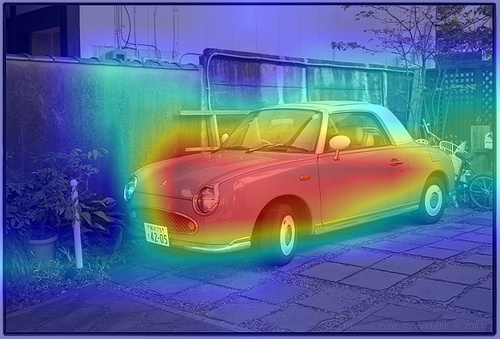
\includegraphics[width=0.23\textwidth]{figures/qualitative_analysis/test_cam/2010_005860_6.jpg} &
    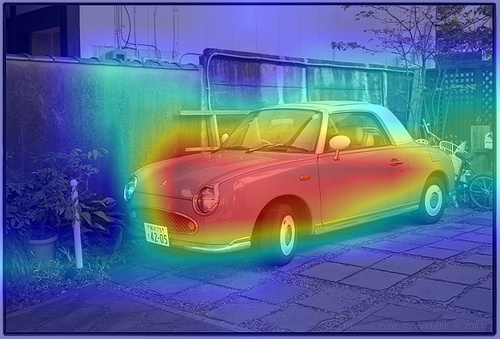
\includegraphics[width=0.23\textwidth]{figures/qualitative_analysis/test_cam/2010_005860_6.jpg} &
    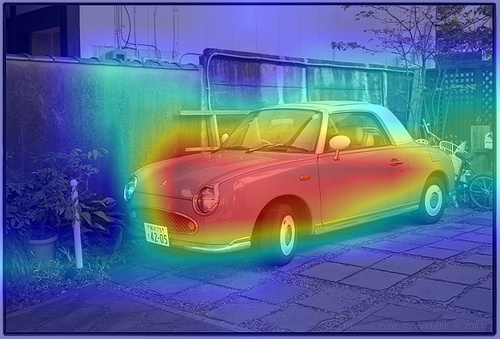
\includegraphics[width=0.23\textwidth]{figures/qualitative_analysis/test_cam/2010_005860_6.jpg} \\

    % Second example
    \textbf{Dog} &
    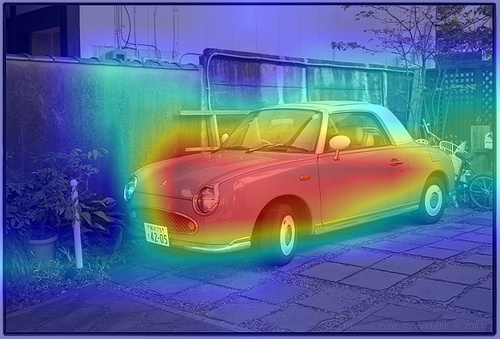
\includegraphics[width=0.23\textwidth]{figures/qualitative_analysis/test_cam/2010_005860_6.jpg} &
    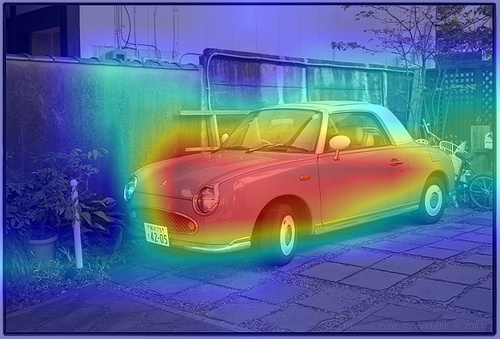
\includegraphics[width=0.23\textwidth]{figures/qualitative_analysis/test_cam/2010_005860_6.jpg} &
    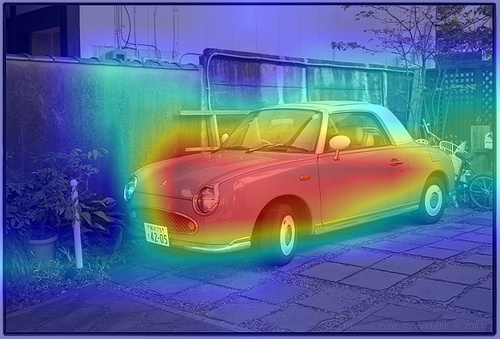
\includegraphics[width=0.23\textwidth]{figures/qualitative_analysis/test_cam/2010_005860_6.jpg} \\
  \end{tabular}

  \caption{Qualitative comparison of CAMs between WeCLIP and our UniCL-AffSeg on PASCAL VOC 2012 \textit{test} set. The class label for each image is shown on the left.}
  \label{fig:qualitative_comparison_cam_test}
\end{figure}

\begin{figure}[ht]
  % Pseudo-labels
  \begin{tabular}{cccc}
    (a) Input & (b) GT & (c) WeCLIP & (d) Ours \\

    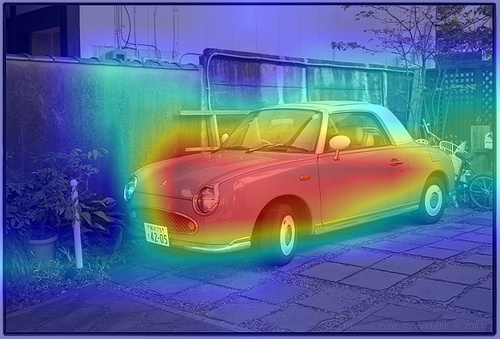
\includegraphics[width=0.22\textwidth]{figures/qualitative_analysis/test_cam/2010_005860_6.jpg} &
    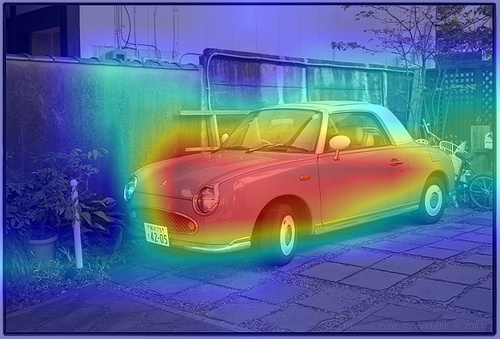
\includegraphics[width=0.22\textwidth]{figures/qualitative_analysis/test_cam/2010_005860_6.jpg} &
    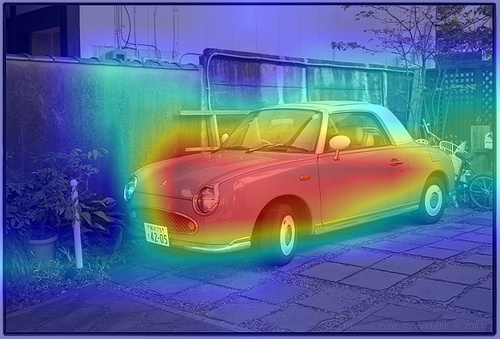
\includegraphics[width=0.22\textwidth]{figures/qualitative_analysis/test_cam/2010_005860_6.jpg} &
    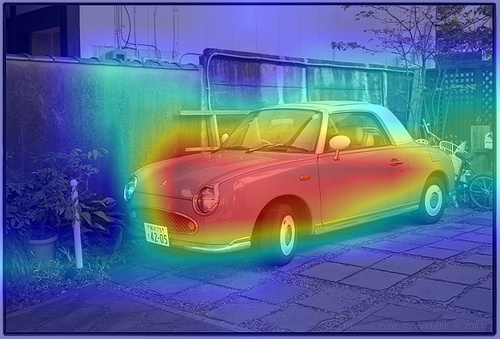
\includegraphics[width=0.22\textwidth]{figures/qualitative_analysis/test_cam/2010_005860_6.jpg} \\
  \end{tabular}

  \caption{Qualitative comparison of pseudo-labels between WeCLIP and our UniCL-AffSeg on PASCAL VOC 2012 \textit{test} set.}
  \label{fig:qualitative_comparison_pseudolabel_test}
\end{figure}


\subsection{Observations}


\subsection{Summary}
